\documentclass{beamer}
\usetheme{Boadilla}
\usecolortheme{default}
% \usepackage{pgfpages} % TO DELETE
% \setbeameroption{hide notes} % Only slides
% \setbeameroption{show only notes} % Only notes
\setbeameroption{show notes on second screen=right} % Both
\setbeamertemplate{note page}{\pagecolor{yellow!5}\insertnote}\usepackage{palatino}

\usepackage[utf8]{inputenc}
\usepackage[round]{natbib}



\DeclareMathOperator{\rank}{rank}
\DeclareMathOperator{\erank}{erank}
\DeclareMathOperator{\cl}{cl}
\DeclareMathOperator{\diag}{diag}
\DeclareMathOperator{\spn}{span}
% \newtheorem{theorem}{Theorem}
\newtheorem{assumption}{Assumption}
% \newtheorem{definition}{Definition}
\newtheorem{observation}{Observation}
% \newtheorem{corollary}{Corollary}
% \newtheorem{lemma}{Lemma}
\usepackage{dsfont}
\newcommand{\onefunc}{\mathds{1}}
\newcommand{\din}{{d_{\text{in}}}}
\newcommand{\dhid}{{d_{\text{hidden}}}}
\newcommand{\dout}{{d_{\text{out}}}}
\newcommand{\eps}{\epsilon}
\newcommand{\TODO}{\Red{TODO}}
\newcommand{\abs}[1]{\left|{#1}\right|}
\newcommand{\tr}[1]{\text{Tr}\left({#1}\right)}
\newcommand{\vect}[1]{\text{vec}\left({#1}\right)}
\newcommand{\opt}[1]{#1^\star}
\newcommand{\norm}[2][]{{\left\|{#2}\right\|_{#1}}}
%\newcommand{\norm}[1]{\left\|#1\right\|}
\newcommand{\snorm}[1]{\|#1\|} %small norm
\renewcommand{\angle}[2]{\measuredangle \left( #1, #2 \right)}
\newcommand{\bigangle}[2]{\measuredangle \left\big( #1, #2 \right\big)}
\newcommand{\Red}[1]{\colorbox{red}{#1}}
\newcommand{\set}[1]{\left\{{#1}\right\}}

\newcommand{\ba}{\mathbf{a}}
\newcommand{\be}{\mathbf{e}}
\newcommand{\bx}{\mathbf{x}}
\newcommand{\bw}{\mathbf{w}}
\newcommand{\bg}{\mathbf{g}}
\newcommand{\bb}{\mathbf{b}}
\newcommand{\bu}{\mathbf{u}}
\newcommand{\bv}{\mathbf{v}}
\newcommand{\bz}{\mathbf{z}}
\newcommand{\bc}{\mathbf{c}}
\newcommand{\br}{\mathbf{r}}
\newcommand{\bd}{\mathbf{d}}
\newcommand{\bp}{\mathbf{p}}
\newcommand{\bh}{\mathbf{h}}
\newcommand{\by}{\mathbf{y}}
\newcommand{\bn}{\mathbf{n}}
\newcommand{\bs}{\mathbf{s}}
\newcommand{\bq}{\mathbf{q}}
\newcommand{\bmu}{\boldsymbol{\mu}}
\newcommand{\balpha}{\boldsymbol{\alpha}}
\newcommand{\bbeta}{\boldsymbol{\beta}}
\newcommand{\btau}{\boldsymbol{\tau}}
\newcommand{\bxi}{\boldsymbol{\xi}}
\newcommand{\blambda}{\boldsymbol{\lambda}}
\newcommand{\bepsilon}{\boldsymbol{\epsilon}}
\newcommand{\bsigma}{\boldsymbol{\sigma}}
\newcommand{\btheta}{{\boldsymbol{\theta}}}
\newcommand{\bomega}{\boldsymbol{\omega}}
\newcommand{\Xcal}{\mathcal{X}}

\newcommand{\co}{{\cal O}}
\newcommand{\ca}{{\cal A}}
\newcommand{\cb}{{\cal B}}
\newcommand{\cd}{{\cal D}}
\newcommand{\cdb}{{\cal D}^{\rm b}}
\newcommand{\cc}{{\cal C}}
\newcommand{\ck}{{\cal K}}
\newcommand{\cq}{{\cal Q}}
\newcommand{\ce}{{\cal E}}
\newcommand{\ct}{{\cal T}}
\newcommand{\cg}{{\cal G}}
\newcommand{\ch}{{\cal H}}
\newcommand{\cm}{{\cal M}}
\newcommand{\ci}{{\cal I}}
\newcommand{\cj}{{\cal J}}
\newcommand{\cw}{{\cal W}}
%\newcommand{\cl}{{\cal L}}
\newcommand{\cf}{{\cal F}}
\newcommand{\cv}{{\cal V}}
\newcommand{\cp}{{\cal P}}
\newcommand{\cu}{{\cal U}}
\newcommand{\cx}{{\cal X}}
\newcommand{\cy}{{\cal Y}}
\newcommand{\cz}{{\cal Z}}
\newcommand{\cs}{{\cal S}}
\newcommand{\cn}{{\cal N}}
\newcommand{\calr}{{\cal R}}

\newcommand{\bbs}{{\mathbb S}}
\newcommand{\reals}{{\mathbb R}}
\newcommand{\nat}{{\mathbb N}}
\newcommand{\integers}{{\mathbb Z}}
\newcommand{\complex}{{\mathbb C}}
\newcommand{\zero}{{\mathbf{0}}}




\title[Implicit Bias: Rank Min. in ReLU Networks]{Implicit Regularization Towards Rank Minimization in ReLU Networks}
\author[Nadav Timor]{
    by Nadav Timor\newline
    Advisor: Prof. Ohad Shamir
}
\institute[Weizmann Institute]{Weizmann Institute of Science}
\date[January 2022]{January 2022}
\logo{
\includegraphics[height=.75cm]{WeizmannLogo.png}}



\begin{document}



\frame{\titlepage}

\begin{frame}
    \frametitle{Implicit~Regularization Towards Rank~Minimization\\in ReLU~Networks}
    A joint paper under review @ ICML 2022,\\
    w/ Gal Vardi and Ohad Shamir.
\end{frame}



\section{Introduction}

\subsection{The problem}

\begin{frame}{Intro: The problem}{Generalization despite overparameterization}
    \pause
    \newline
    If \#[learnable parameters] $>>$ \#[training examples]:
    \pause
    \begin{columns}
        \column{0.5\textwidth}
        \begin{itemize}
            \item \alert{Many global minima}\\
            (w/ $0$ training loss).
            \pause
            \item Might \alert{overfit}.
            \pause
            \begin{itemize}
                \item Popular solution:\\explicit regularization.
            \end{itemize}
        \end{itemize}
        \column{0.5\textwidth}
        \begin{figure}
        \centering
            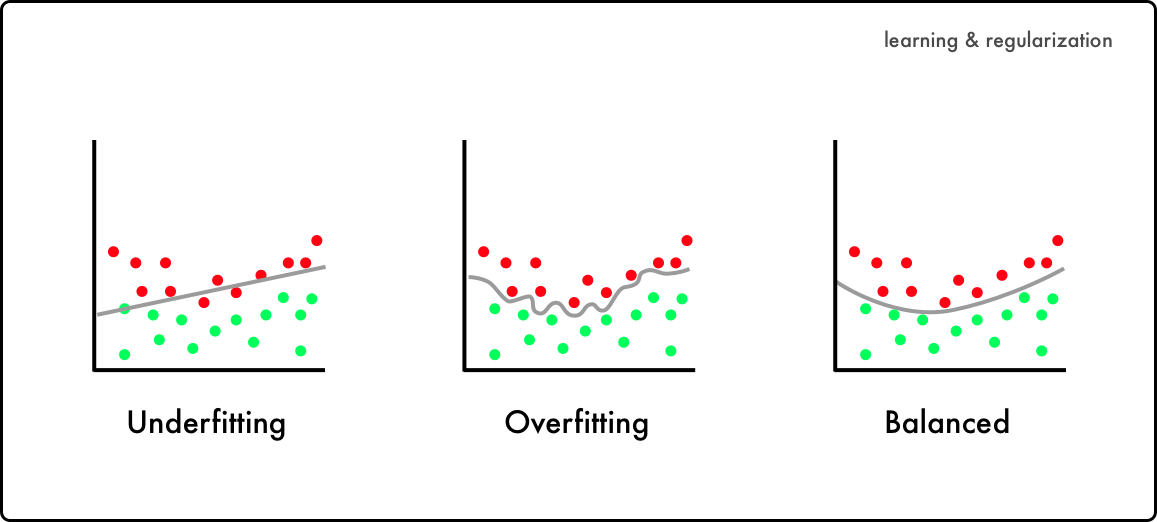
\includegraphics[width=6cm]{figures/overfitting.png}
            % \caption{}
            % \label{fig:overfitting}
        \end{figure}
    \end{columns}
    \pause
    \begin{block}{Phenomenon in practice (\cite{zhang2017understanding})}
        Networks trained \alert{w/o explicit~regularization} generalize well.
        \newline
        \newline
        (despite \#[learnable parameters] $>>$ \#[training examples])
    \end{block}
    \pause
    \textbf{Q:} How?\\
    \pause
    \textbf{Possible A:} ``implicit regularization'' (or ``implicit bias'').
    
    \note{
        \alert{If asked:}
        \begin{enumerate}
            \item \cite{zhang2017understanding}:\\
            Large CNNs, trained w/ stochastic~gradient~methods\\
            fit a random~labeling (of the training~data), or even completely~unstructured random~noise.\\
            Unaffected by explicit~regularization.
        \end{enumerate}
    }
\end{frame}


\subsection{Previous work}
\subsubsection{Implicit regularization in linear networks}

\begin{frame}{Intro: Previous work}{Implicit regularization in linear networks}
    \pause
    \begin{definition}[fully-connected~neural~network]
        A fully-connected~neural~network $N_\btheta$ of depth~$k \geq 2$ is parameterized by a collection~$\btheta := [W^{(\ell)}]_{\ell=1}^k$ of weight~matrices\\
        ($\forall \ell \in [k] : W^{(\ell)} \in \reals^{d_\ell \times d_{\ell-1}}$), and computes a function $N_\btheta : \reals^\din \to \reals^\dout$:
        \[
            N_\btheta(\bx) := 
            \onslide<5->{W^{(k)}}
                \onslide<4->{\sigma\Big( W^{(k-1)} \ldots }
                    \onslide<3->{\sigma\Big( W^{(2)}~} 
                        \sigma\Big( W^{(1)} \bx \Big) 
                    \onslide<3->{\Big)}
                \onslide<4->{ \Big)} 
            \onslide<5->{\Big)}
            , \forall \bx
        \]
        where $\sigma:\reals \to \reals$ is an activation~function that acts coordinate-wise.
    \end{definition}
    \onslide<6->{
        \begin{description}
            \item[fully-connected \emph{linear} neural~network] $N_\btheta$, where $\sigma$ is the identity.
            \item[fully-connected \emph{ReLU} neural~network] $N_\btheta$, where $\sigma(z) := \max\set{0, z}$.
        \end{description}
    }
    \onslide<7->{
        \begin{block}{Well-studied test-bed: Matrix Factorization}
            What is the implicit regularization of training a depth-2 linear network w.r.t. square loss?\\
            (find $W^{(2)}W^{(1)}\bx_i = W^* \bx_i, \forall i \in [n]$.)
        \end{block}
    }
\end{frame}



\begin{frame} %{Intro: Previous work}{Implicit regularization in linear networks}
    \begin{definition}[square loss]
        Given a network $N_\btheta$ and a dataset $\{(\bx_i,\by_i)\}_{i=1}^n \subseteq \reals^\din \times \reals^\dout$,
        \begin{align} \label{eq:objective}
        	 L_{X,Y}(\btheta) 
        	 := \frac{1}{2} \sum_{i=1}^n \norm{N_\btheta(\bx_i) - \by_i}^2
        	 = \frac{1}{2} \norm{N_\btheta(X) - Y}_F^2~.
        \end{align}
        $(X,Y) \in \reals^{\din \times n} \times \reals^{\dout \times n}$ are the corresponding data matrices.
    \end{definition}
    \pause
    \begin{itemize}
        \item Overparameterization $\Rightarrow$
        \pause
        \begin{itemize}
            \item $\min_\btheta L(\btheta)=0$.
            \pause
            \item $L$ has multiple (or even infinitely many) global minima.
        \end{itemize}
    \end{itemize}
    \begin{definition}[gradient flow (GF) w.r.t. square loss]
        Let~$\btheta(t)$ be the trajectory of GF. Starting from $\btheta(0)$, the dynamics is given by $\frac{d \btheta(t)}{dt} = -\nabla L_{X,Y}(\btheta(t))$.
    \end{definition}
    \begin{itemize}
        \item Behaves as GD w/ an infinitesimally small step~size.
        \pause
        \item GF \emph{converges} $\Leftrightarrow \lim_{t \to \infty}\btheta(t)$~exists. \pause $\btheta(\infty) := \lim_{t \to \infty}\btheta(t)$.
        \pause
        \item We assume $\sigma'(0) = 0$ for convenience.
    \end{itemize}
    
    \note{
        \begin{enumerate}
            \item Our assumption that $\sigma'(0) = 0$:\\
            Practical implementations of gradient~methods define $\sigma'(0) \in [0,1]$.
        \end{enumerate}
    }
\end{frame}



\begin{frame}{Implicit regularization in linear~networks/matrix~factorization}
    \pause
    \begin{block}{\cite{gunasekar2018implicit}’s conjecture}
        The implicit~regularization in matrix~factorization can be characterized by the \alert{nuclear~norm} of the corresponding linear~predictor.
    \end{block}
    \begin{itemize}
        \item This conjecture was further studied in a string of works (e.g., \cite{belabbas2020implicit,arora2019implicit,razin2020implicit}) and was \alert{formally refuted} by \cite{li2020towards}.
    \end{itemize}
    \pause
    \item \cite{razin2020implicit} conjectured that the implicit~regularization in matrix~factorization can be explained by rank~minimization, and also hypothesized that some notion of rank~minimization may be key to explaining generalization in deep~learning.
    \pause
    \begin{itemize}
        \item \cite{li2020towards} established evidence that the implicit~regularization in matrix~factorization is a heuristic for rank~minimization.
    \end{itemize}
\end{frame}



\AtBeginSection[]
{
    \begin{frame}{Table of Contents}
        \tableofcontents[currentsection]
    \end{frame}
}



\subsubsection{Implicit regularization in ReLU networks}




\section{Results}

\begin{frame}{Sample frame title}

In this slide, some important text will be
\alert{highlighted} because it's important.
Please, don't abuse it.

\begin{block}{Remark}
Sample text
\end{block}

\begin{alertblock}{Important theorem}
Sample text in red box
\end{alertblock}

\begin{examples}
Sample text in green box. The title of the block is ``Examples".
\end{examples}
\end{frame}


\section*{References}
\begin{frame}{References}
    \bibliography{bib}
    \bibliographystyle{abbrvnat}    
\end{frame}

\end{document}